\section{Evaluation}
\label{sec:eval}

%~\todo{needs to go through the text and make sure they are consistent with the figures!!!}
In this section, we analyze the performance of Presto for (i) synthetic workloads, (ii)
trace-driven workloads, (iii) workloads containing north-south cross traffic, and (iv) failures.
All tests are run on the topology in Figure~\ref{macro_evaluation_topology}.
\begin{figure}[!t]
        \centering
  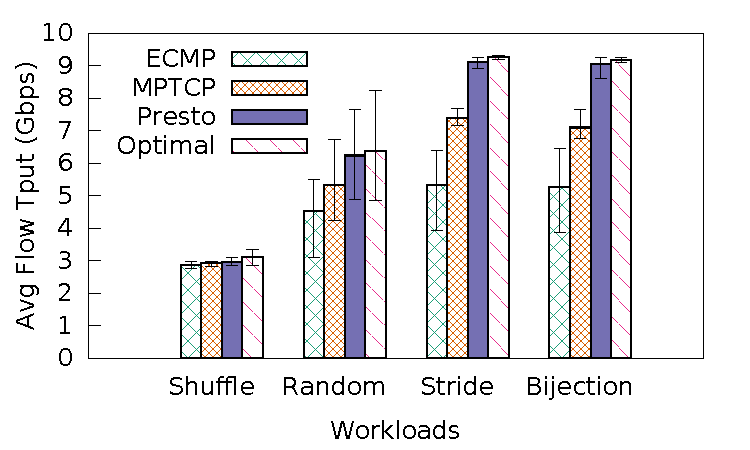
\includegraphics[width=0.5\textwidth]{presto/figures/macro/stride/macro_compare_tput_witherrbar.pdf}
        \caption{Elephant flow throughput for ECMP, MPTCP, Presto and Optimal in shuffle, random, stride and random bijection workloads.}
        \label{macro_evaluation_tput}
\end{figure}



\begin{figure*}[!t]
        \centering
	\begin{subfigure}[b]{0.3\textwidth}
                \centering
  		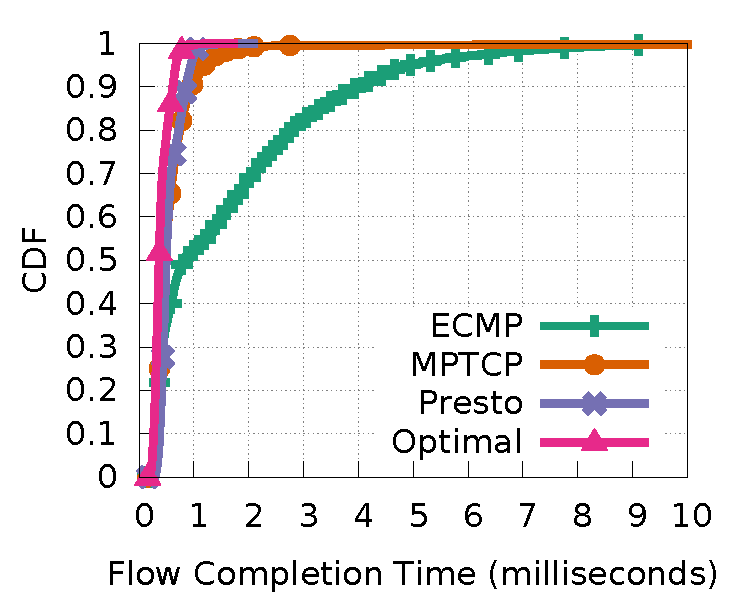
\includegraphics[width=\textwidth]{presto/figures/macro/stride/macro_compare_fct_stride_mice.pdf}
        	\caption{Stride}
        	\label{macro_evaluation_fct_stride}
	\end{subfigure}
	\begin{subfigure}[b]{0.3\textwidth}
                \centering
		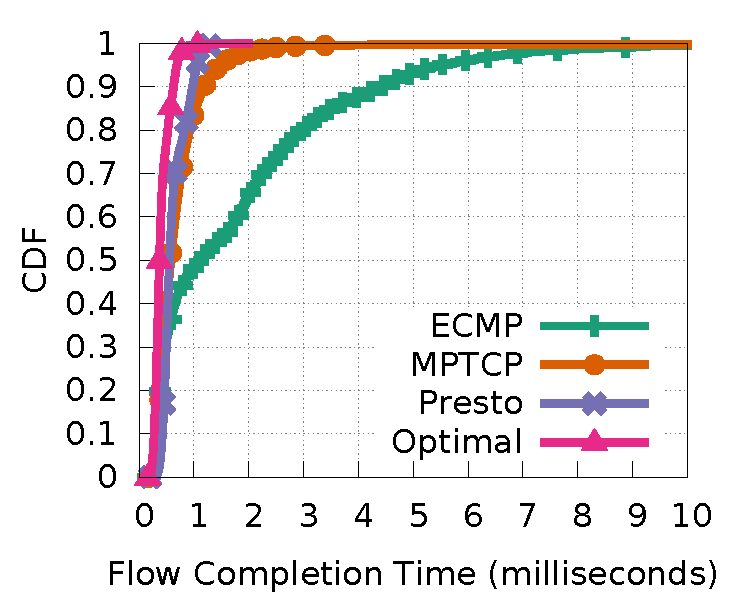
\includegraphics[width=\textwidth]{presto/figures/macro/bijection/macro_compare_fct_bijection_mice.pdf}
        	\caption{Random Bijection}
        	\label{macro_evaluation_fct_bijection}
	\end{subfigure}
        %\begin{subfigure}[b]{0.225\textwidth}
        %        \centering
	%	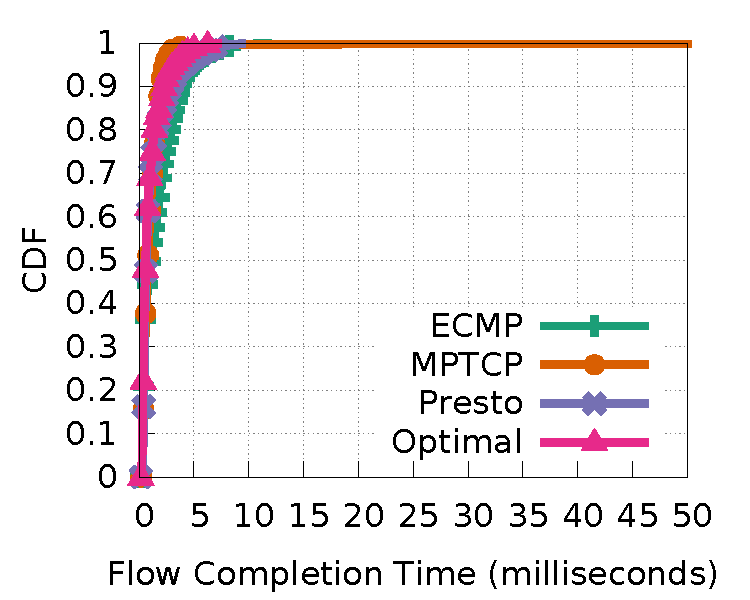
\includegraphics[width=\textwidth]{presto/figures/macro/random/macro_compare_fct_random_mice.pdf}
        %	\caption{Random}
        %	\label{macro_evaluation_fct_random}
	%\end{subfigure}
        \begin{subfigure}[b]{0.3\textwidth}
                \centering
		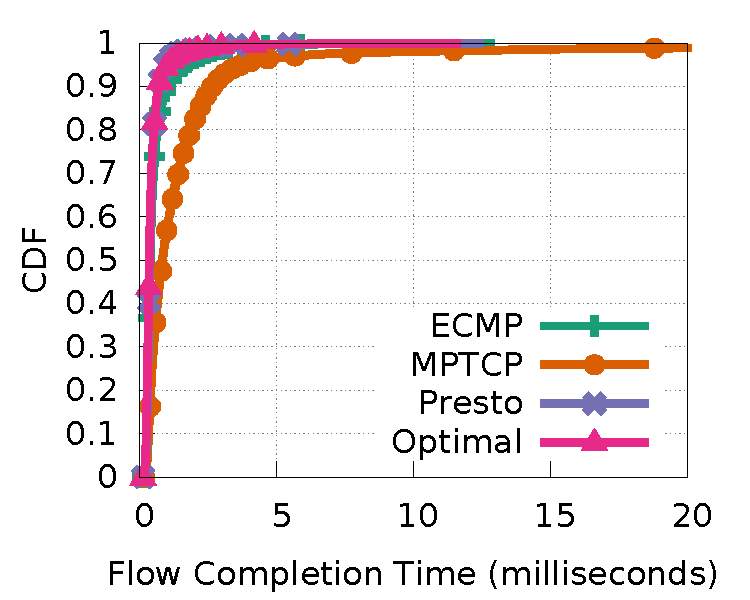
\includegraphics[width=\textwidth]{presto/figures/macro/shuffle/macro_compare_fct_shuffle_mice.pdf}
        	\caption{Shuffle}
        	\label{macro_evaluation_fct_shuffle}
	\end{subfigure}
	\caption{Mice FCT of ECMP, MPTCP, Presto and Optimal in stride, random bijection, and shuffle workloads.}
	\label{macro_evaluation_fct}
\end{figure*}

\tightparagraph{Synthetic Workloads}
Figure~\ref{macro_evaluation_tput} 
shows the average throughputs of elephant flows in the shuffle, random, stride and random bijection workloads.
Presto's throughput is within 1-4\% of Optimal over all workloads.
For the shuffle workload, ECMP, MPTCP, Presto and Optimal show similar results 
because the throughput is mainly bottlenecked at the receiver. 
%due to several servers sending to the same receiver.
In the non-shuffle workloads, Presto improves upon ECMP by 38-72\% and improves
upon MPTCP by 17-28\%.
%Compared with ECMP, 
%Presto improves throughput by 71\% (stride), 72\% (random bijection) and 38\% (random).
%Presto also outperforms MPTCP with throughput improvements of 23\% (stride), 28\% (random bijection) and 
%17\% (random).
%In all the workloads, Presto's throughput outperforms MPTCP.

Figure~\ref{macro_evaluation_fct} shows a CDF of the mice flow completion time (FCT) for each workload.
The stride and random bijection workloads are non-blocking, and hence the latency of Presto
closely tracks Optimal: the 99.9$^{th}$ percentile FCT for Presto is within 350 $\mu$s for these workloads.
MPTCP and ECMP suffer from congestion, and therefore the tail FCT is much worse than Presto: ECMP's 99.9$^{th}$ percentile
FCT is over 7.5x worse ($\sim$11ms) and MPTCP experiences timeout (because of higher loss
rates and the fact that small sub-flow window sizes from small flows can increase the chances of timeout~\cite{dc-mptcp}). We used the Linux default timeout (200 ms) and trimmed graphs for clarity.
The difference in the random and shuffle workloads is less pronounced (we omit random due to space constraints).
In these workloads elephant flows can collide on the last-hop output port,
and therefore mice FCT is mainly determined by queuing latency. In shuffle, the 99.9$^{th}$ percentile FCT for ECMP, Presto and Optimal
are all within 10\% (MPTCP again experiences TCP timeout) and in random, the 99.9$^{th}$ percentile FCT of Presto is within 25\% of Optimal while ECMP's 
is 32\% worse than Presto.


%%the following are combined into one figure
\iffalse
\begin{figure}[!t]
        \centering
  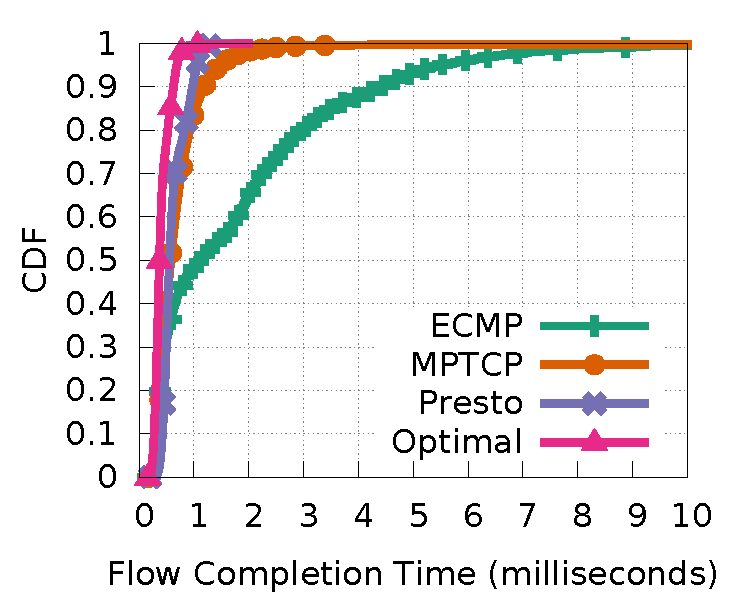
\includegraphics[width=0.45\textwidth]{presto/figures/macro/bijection/macro_compare_fct_bijection_mice.pdf}
        \caption{Macro evaluation - flow completiom time in Random Bijection workload}
        \label{macro_evaluation_fct_bijection}
\end{figure}

\begin{figure}[!t]
        \centering
  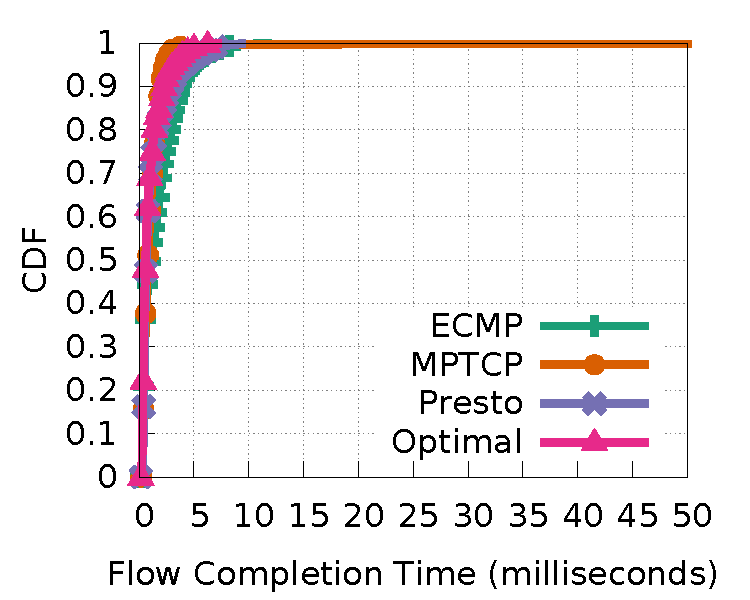
\includegraphics[width=0.45\textwidth]{presto/figures/macro/random/macro_compare_fct_random_mice.pdf}
        \caption{Macro evaluation - flow completiom time in Random workload}
        \label{macro_evaluation_fct_random}
\end{figure}


\begin{figure}[!t]
        \centering
  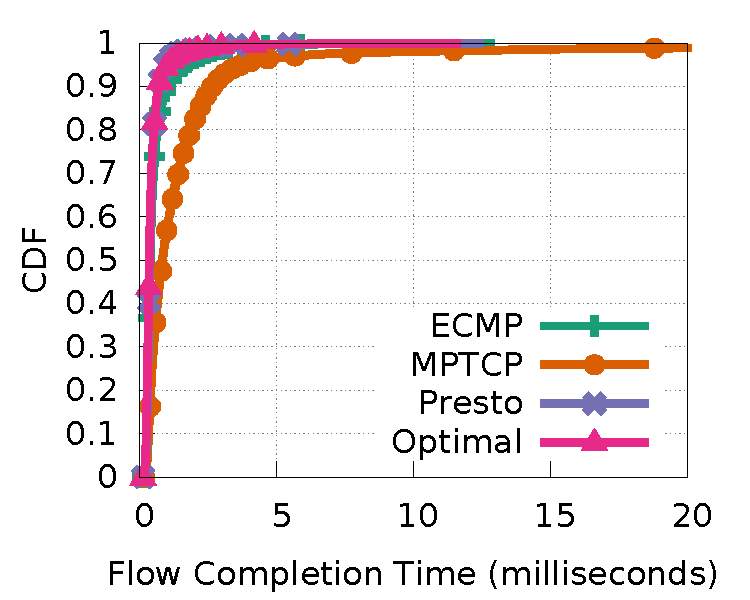
\includegraphics[width=0.45\textwidth]{presto/figures/macro/shuffle/macro_compare_fct_shuffle_mice.pdf}
        \caption{Macro evaluation - flow completiom time in Shuffle workload}
        \label{macro_evaluation_fct_shuffle}
\end{figure}

\fi

\iffalse
\begin{table}[!htb]
\begin{center}
\begin{tabular}{ |c|c|c|c|c| } 
 \hline
 Shuffle & ECMP & MPTCP & Presto & Optimal \\
 \hline 
 Median & 401 & 874 & 387 & 369  \\ 
 90\%   & 1037 & 2664 & 726 & 712 \\
 99\%   & 3373 & 21600  & 2447 & 2446 \\ 
 99.9\% & 12830 & 206ms & 12480 & 11714 \\
 %99.99\% & 204.1ms & - & 204.1ms & 203.6ms \\
 \hline

\end{tabular}
\caption{Macro evaluation - A close look of flow completiom time in Shuffle workload}
        \label{macro_evaluation_fct_shuffle_closelook}
\end{center}
\end{table}

\begin{table}[!htb]
\begin{center}
\begin{tabular}{ |c|c|c|c|c| }
 \hline
 Random & ECMP & MPTCP & Presto & Optimal \\
 \hline
 Median & 1008 & 780 & 648 & 595  \\
 90\%   & 3815 & 1918 & 2850 & 2297 \\
 99\%   & 7852 & 3380  & 6900 & 4936 \\
 99.9\% & 11784 & 202ms & 9372 & 7127 \\
% 99.99\% & 11677 & - & 16591 & 200ms \\
 \hline

\end{tabular}
\caption{Macro evaluation - A close look of flow completiom time in Random workload}
        \label{macro_evaluation_fct_random_closelook}
\end{center}
\end{table}

\fi

%%% trace-driven workload, MSR, scaling factor =10
\begin{table}[!tb]
\begin{center}
\begin{tabular}{ |c|c|c|c| }
 \hline
 Percentile & ECMP & Optimal &Presto \\
 \hline
 50\%   & $1.0$ & $-12\%$ & $-9\%$   \\
 90\%   & $1.0$ & $-34\%$ & $-32\%$  \\
 99\%   & $1.0$ & $-63\%$  & $-56\%$ \\
 99.9\% & $1.0$ & $-61\%$ & $-60\%$  \\
 \hline

\end{tabular}
\caption{Mice ($<$100KB) FCT in trace-driven workload~\cite{kandula2009nature}. Negative numbers imply shorter FCT.}
        \label{macro_evaluation_MSR_trace_driven}
\end{center}
\end{table}

\tightparagraph{Trace-driven Workload}
We evaluate Presto using a trace-driven workload based on traffic patterns measured in~\cite{kandula2009nature}. 
Each server establishes a long-lived TCP connection 
with every other server in the testbed. 
Then each server continuously samples flow sizes and inter-arrival times and each time sends to a random receiver
that is not in the same rack.
%Since 99\% of flows are less than 4MB in the distribution, 
We scale the flow size distribution by a factor of 10 to emulate a heavier workload. 
Mice flows are defined as flows that are less than 100 KB in size, and elephant flows are defined as flows
that are greater than 1 MB. The mice FCT, normalized to ECMP, 
is shown in Table~\ref{macro_evaluation_MSR_trace_driven}. 
Compared with ECMP, Presto has similar performance at the 50$^{th}$ percentile but reduces the 99$^{th}$ and 99.9$^{th}$ percentile FCT by 56\% and 60\%, respectively. 
Note MPTCP is omitted because its performance was quite unstable in workloads
featuring a large number of small flows.
The average elephant throughput (not shown) for Presto tracks Optimal (within 2\%), and improves upon ECMP by over 10\%.


\begin{table}[!htb]
\begin{center}
\begin{tabular}{ |c|c|c|c|c| }
 \hline
% Percentile & 50\% & 90\% & 99\% & 99.9\% \\
% \hline
% ECMP & 1.0 & 1.0 & 1.0 & 1.0  \\
% N-block   & 66\% & 17\% & 11\% & 9\% \\
% Presto    & 80\% & 21\% & 14\% & 10\% \\
% MPTCP     & 88\% & 27\% & 27\% & TIMEOUT \\

 Percentile & ECMP & Optimal & Presto & MPTCP \\
 \hline
 50\%       & 1.0 & $-34$\%     & $-20$\%   & $-12$\% \\
 90\%       & 1.0 & $-83$\%     & $-79$\%   & $-73$\% \\
 99\%       & 1.0 & $-89$\%     & $-86$\%   & $-73$\% \\
 99.9\%     & 1.0 & $-91$\%      & $-87$\%   & TIMEOUT \\

 \hline
\end{tabular}
\caption{FCT comparison (normalized to ECMP) with ECMP load balanced north-south traffic. Optimal means all the hosts are attached to a single  switch.}
	\label{macro_evaluation_north_south_traffic}
\end{center}
\end{table}


\tightparagraph{Impact of North-South Cross Traffic}
Presto load balances on "east-west" traffic in the datacenter, \ie{}, traffic
originating and ending at servers in the datacenter. 
In a real datacenter environment "north-south" traffic (\ie{}, traffic with an endpoint outside the datacenter)
must also be considered. 
%Ideally, north-south traffic should be load balanced by ECMP because of 
%reordering concerns at the end user. 
%However, east-west traffic typically dominates (75\% according to~\cite{east-west}). 
To study the impact of north-south traffic on Presto, we attach an additional server to 
each spine switch in our testbed to emulate remote users. 
The 16 servers establish a long-lived TCP connection with each remote user. 
Next, each server starts a flow to a random remote user every 1 millisecond. This emulates  
the behavior of using ECMP to load balance north-south traffic.
The flow sizes for north-south traffic are based on the distribution measurement in~\cite{he2013next}. 
The throughput to remote users is limited to 100Mbps to emulate the limitation of an Internet WAN. 
Along with the north-south flows, 
a stride workload is started to emulate the east-west traffic. 
The east-west mice FCT is shown in Table~\ref{macro_evaluation_north_south_traffic} (normalized to ECMP). 
ECMP, MPTCP, Presto, and Optimal's average throughput is 
5.7, 7.4, 8.2, and 8.9Gbps respectively. 
The experiment shows Presto can gracefully co-exist with north-south cross traffic
in the datacenter.


%%%failure handling experiments

\begin{figure}[!t]
        \centering
  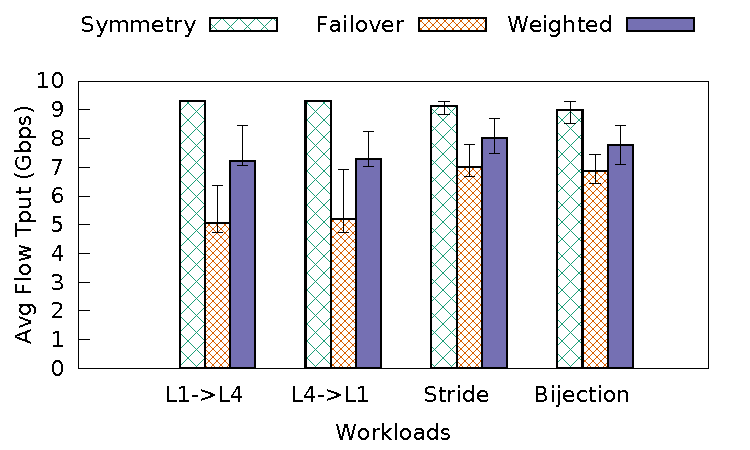
\includegraphics[width=0.5\textwidth]{presto/figures/failure_handling/failover_compare_tput_witherrbar.pdf}
        \caption{Presto's throughput in symmetry, fast failover and weighted multipathing stages for different workloads.}
        \label{failover_compare_tput}
\end{figure}

\begin{figure}[!t]
        \centering
  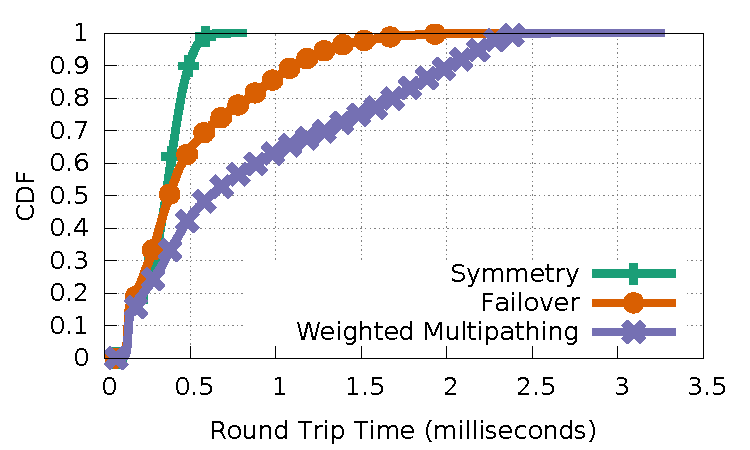
\includegraphics[width=0.5\textwidth]{presto/figures/failure_handling/failover_compare_sockperf_bijection_mice.pdf}
        \caption{Presto's RTT in symmetry, fast failover and weighted multipathing stages in  random bijection workload.}
        \label{failover_compare_sockperf_bijection}
\end{figure}

\tightparagraph{Impact of Link Failure}
Finally, we study the impact of link failure.
Figure~\ref{failover_compare_tput} compares the throughputs of
Presto when %under different stages of loss recovery when 
the link between spine switch S1 and leaf switch L1 goes down.
Three stages are defined: symmetry (the link is up), failover (hardware fast-failover moves traffic from S1 to S2), and weighted (the controller
learns of the failure and prunes the tree with the bad link).
Workload L1$\rightarrow$L4 is when each node connected to L1 sends to one node in L4 (L4$\rightarrow$L1 is the opposite).
Despite the asymmetry in the topology, Presto still achieves reasonable average throughput at 
each stage.
Figure~\ref{failover_compare_sockperf_bijection} shows the round trip time of
each stage in a random bijection workload. 
Due to the fact that the network is no longer non-blocking after the link failure,
failover and weighted multipathing stages have larger round trip time.



\iffalse
\begin{enumerate}
\item Clos-network, macro. ECMP, MPTCP, Presto and Optimal.
\begin{enumerate}
	\item Workloads: Take from Planck and Hedera. Can do MSR trace-based.
	\item Throughput, fairness, latency (maybe loss). Link utilization?
\end{enumerate}

\item Fat tree, macro. ECMP, MPTCP, Presto and Optimal.
\begin{enumerate}
        \item Workloads: Take from Planck and Hedera. Can do MSR trace-based.
        \item Throughput, fairness, latency (maybe loss). Link utilization?
\end{enumerate}


\item Vary flow sizes. Idea is that we can work on very small elephants.

\item Failure: backbone switch fails, aggregate switch fails, ToR switch fails, link fails, ...

\item CONGA uses incast, should we check?

\item Maybe this belongs in micro: ECMP vs shadowMAC for multipathing.

\end{enumerate}
\fi
